\documentclass[10pt,twocolumn,letterpaper]{article}

\usepackage{iccv}
\usepackage{times}
\usepackage{epsfig}
\usepackage{graphicx}
\usepackage{amsmath}
\usepackage{amssymb}
\usepackage{indentfirst}

% Include other packages here, before hyperref.

% If you comment hyperref and then uncomment it, you should delete
% egpaper.aux before re-running latex.  (Or just hit 'q' on the first latex
% run, let it finish, and you should be clear).
\usepackage[breaklinks=true,bookmarks=false]{hyperref}
\setkeys{Gin}{width=\columnwidth}
\graphicspath{{pictures/}}
\iccvfinalcopy % *** Uncomment this line for the final submission

\def\iccvPaperID{****} % *** Enter the ICCV Paper ID here
\def\httilde{\mbox{\tt\raisebox{-.5ex}{\symbol{126}}}}

% Pages are numbered in submission mode, and unnumbered in camera-ready
%\ificcvfinal\pagestyle{empty}\fi
\setcounter{page}{1}
\begin{document}

%%%%%%%%% TITLE
\title{A Review Of Immersive Scientific Visualization}

\author{Zhongyuan Yu\\
{\tt\small algoyu@163.com}
% For a paper whose authors are all at the same institution,
% omit the following lines up until the closing ``}''.
% Additional authors and addresses can be added with ``\and'',
% just like the second author.
% To save space, use either the email address or home page, not both
\and
Stefanie Krell\\
{\tt\small stefanie.krell@mailbox.tu-dresden.de}
}

\maketitle
%\thispagestyle{empty}


%%%%%%%%% BODY TEXT
\section{Introduction}
Scientific Visualization is the visualization of scientific phenomena. That includes the visualization of flow, particles, terrain, volume and tensors. The purpose is to enable scientists to understand, illustrate and get insight from their data. The data is often very large and most of the time in 3D. The use of stereoscopic images can improve the depth cue and the perception of the spatial relationships which might be crucial for scientist when analyzing data.

\setlength{\parindent}{1pc}
Virtual reality can give a sense of presence or immersion in 3D environment. It is a class of computer-controlled multisensory communication technologies that allow more intuitive interactions with data and involve human senses in new ways. Nowadays head mounted displays (HMDs) like Oculus Rift1 or HTC Vive2 are widely available.There are also VR systems like the CAVE: an immersive virtual reality environment where projectors are directed to between three and six of the walls of a room-sized cube. It uses motion capture system, which records the real time position of the user, for interaction. When using VR for Scientific Visualization, scientists can explore the data in ways which might lead to insights they would otherwise not get.
\section{Point Cloud Visualization}
\subsection{Overview}
In this project \cite{discher_point-based_2018} they utilized a multi-pass rendering pipeline to visualize 3D Point clouds with different rendering techniques. 3D point clouds are datasets which come from 3D scans e.g. via Airborne Laser scanning or Terrestrial Laser scanning or mobile Laserscanning. They are used in areas like …
Real time rendering of 3d points clouds allows for interactive exploring of real-world assets, sites or regions. In Virtual reality the applications have to cope with very high framerates ( 90fps as opposed to 30-60fps) and high sensivity to any kind of visual artifacts which are typical for showing 3D Point Clouds(e.g holey surfaces and visual clutter). It is a project that allows for exploration of 3D point clouds with CR devices such as HTC Vive or Oculus Rift. It was tested with up to 2.6 billion points. The goal of this project was to show the scalability and practicability of the approach.
There are similar approaches out their like ….
This project is quite different to the other papers explained in this review.
\begin{figure}
	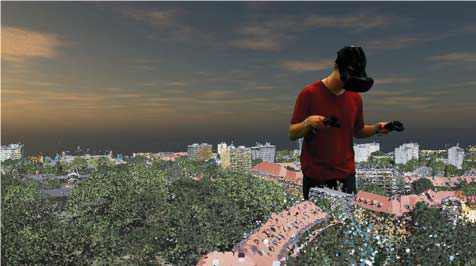
\includegraphics{pointcloud_1.png}
	\caption{Point-cloud Visulization on HTC Vive of an Airborne scan of a city}
	\label{img:pointcloud_1}
\end{figure}

\subsection{Rendering}
The rendering system of the project consists of 3 basic steps: data subset selection, point cloud rendering and image-based post processing.

\setlength{\parindent}{1pc}Data subselection is necessary because presentation and interactive visualization of 3D point clouds have to deal with the massive amount of data which generally exceeds available CPU and GPU capabilities. That is why out-of-core rendering concepts and spatial data structures are required. Here they determine the subset on a per-frame basis. Points outside the view frustum are excluded and . As a data structure to provide efficient access they are using kd-trees. This allows for minimal traversal times during rendering and the tree structure is balanced independent of the spatial position of points.

\setlength{\parindent}{1pc}Their next step they called point cloud rendering. The data subset is rendered into g-buffers that combine multiple 2d textures. During runtime it is possible to select different rendering rendering techniques. They implemented three different rendering techniques to evaluate the performance. First one is the Hidden mesh rendering. The actual visible area on screen on VR devices is restricted to a circular area. To prevent a lot of unnecessary fragment shader operations, they used this technique to discard those fragments early on \cite{vlachos_advanced_2015}. Next technique they implemented is the reverse painters algorithm \cite{foley1996computer} which is a GPU-based occlusion culling technique based on early fragment testing. Scene objects should be rendered in order of their distance to the view position for the technique to have a measurable effect. That is done on a per node basis of the kd-tree rather than per point bases to increase performance. Both of these techniques improved the performance but it varies depending on the number of fragments.
The third rendering technique is single-pass stereo rendering which has the goal to reduce the CPU-overhead by rendering both views of right and left eye in a single render pass \cite{johansson2016efficient}. The frame buffer size is doubled and instance rendering is used to prevent duplicated draw calls. This technique proved to be less effective because the main performance bottleneck was the gpu rather than the cpu.


\setlength{\parindent}{1pc}The final step of their rendering pipeline is imaged-based post processing. It operates on previously generated g-buffers. The post processing is necessary because the impressiveness of a scene is negatively effected by any kind of visual artifact one would not expect in the real world. The most noticeable artifacts due to inappropriately sized points are holey appearance of surfaces or visual clutter. One technique they used are adaptive point size which work on a per node basis. For each node they determine its deepest descendant that has been selected for rendering. To all its ancestors the adaptive point size is applied. The point sizes are calculated based on a node’s bounding box rather than its LoD since nodes of the same LoD might still have quit different point densities. But the visual artifacts are not completely removed. [...überarbeiten..]
Another rendering technique they used is Paraboloid rendering \cite{schutz2016potree}. It aims to reduce the visual clutter further by rendering points as paraboloids rather than screen aligned disks. A depth offset is added to fragments. Undesired occlusions are reduced significantly. But it is not compatible with the rendering techniques using early fragment testing. This technique is also quit slow so should only be used carefully.

Also several post processing techniques are applied, Screen space ambient occlusion (SSAO) \cite{mittring2007finding} and eye-dome lighting (EDL) \cite{boucheny2009interactive} add depth cues and highlight silhouettes, blurring [22]
smoothes aliasing and z-fighting. Furthermore remaining holes are filled and two one-dimensional filter kernels \cite{dobrev2010image} instead of a single two dimensional one for a performance speed up, are applied.
The authors of the paper suggest to not use all image improvement techniques as they would slow down the rendering a lot.


\subsection{Interaction}
For interaction they are using controllers. Rotating and scaling of the rendered data is supported. As well as measure distance between points, and selection of applied rendering technique and color.
\subsection{Conclusion}
The multi-pass approach offers a maximum degree of freedom as rendering techniques can be adjusted at runtime. It is highly beneficial for applications in digital documentation, preservation, and presentation of natural and cultural heritage, because it allows user to remotely explore. Future work can focus on performance improvements by distributing the stereo rendering across two separate GPUs.
\section{Tracing Neurons}
\subsection{Overview}
\subsection{Rendering}
\subsection{Interaction}

\section{Molecular Visualization}
\subsection{Overview}
\subsection{Rendering}
\subsection{Interaction}

\section{Visualization of Atomistic Simulations}
\subsection{Overview}
In this project \cite{reda_visualizing_2013} they present an application for interactive visualization and exploration of large-scale atomistic simulations in ultra-resolution immersive environments on CAVE2. Molecular Dynamics is a principle methodology in the study of nanoscale systems in applications of alternative fuel or energy storage. Even though there are a lot of molecular visualization techniques atomistic simulations remain difficult because complex structures with millions of atoms need to be visualized. Here they are using a hybrid representation which combines a ball-and-stick glyph with volumetric surfaces to show the uncertainty in molecular boundaries at the nanoscale.

\subsection{Rendering}
\begin{figure}
	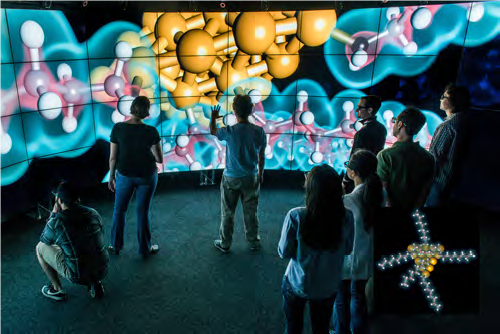
\includegraphics{atomistic_4.png}
	\caption{Visulization of electronic structures}
	\label{img:atomistic}
\end{figure}
For rendering they use volume rendering of electron density field and a ray-cast approach for the ball-and-stick glyphs. To speed up rendering they take an in-core solution. Multiple GPU nodes are used. Stereoscopic rendering is achieved by rendering and interleaving two images separated by the average inter-pupillary distance. To support correct viewing for multiple individuals, they normalized the head orientation when tracking, so that the eyes are always parallel to the screens surface. That might lead to small distortions between the tiles but it is a good compromise.The Ray-cast is done users head to each panel.
As a datastructure to represent ball-and-stick glyphs a uniform 'Macrocells' 3D grid is employed. Each voxel in the grid stores information about all of the atoms and bonds, which are within the cell.
The ray-casting algorithm \cite{Amanatides87afast} traverses each voxel at a discrete level. Because the list of glyphs in a cell is not depth ordered the algorithm has to test every primitive(sphere or cylinder) 



\subsection{Interaction}
CAVE2 provides 3D Navigation using a 6 degrees-of-freedom joystick coupled with head-tracking. The user can fly through the simulation by using a button and by moving/rotating the joystick in the desired direction. The head-tracking provides a user-centered perspective. The user can also adjust the transfer function interactively by the wireless wand or via a tablet. The modification updates the visualization in real-time.

\section{Conclusion}

{\small
\bibliographystyle{unsrt}
\bibliography{reviewbib}
}

\end{document}
